\documentclass[a4paper]{article}
\usepackage{geometry}
 \geometry{
 a4paper,
 total={210mm,297mm},
 left=1.25in,
 right=1.25in,
 top=1.25in,
 bottom=1.25in,
 }
\usepackage{graphicx}
\usepackage{tgpagella}
\usepackage{bbm}
\usepackage{graphicx}
\usepackage{amsmath}
\begin{document}

\title{Convex Optimization Problem Formulation}
\author{Sasank Chilamkurthy \\Ashok Vardhan}
\date{\today}
\maketitle

\section{Problem Statement}
Following is the problem statement, reproduced for reference:
\\
\\
The KReSIT department has $n_1$ rooms. The vector $A$ specifies the number of A/Cs in each room and the vector $F$ specifies the number of fans in each room. Another vector $C$ specifies the number of computer tables in each room, where a computer table is assigned to a specific student/staff. The power consumption of each electrical equipment is as follows (as measured in watts):

fan = $y_f*x_f$, A/C = $y_a*x_a$, computer = $y_c$. 

where $x_f$ is any real number in the range $[0,v_f]$ and $x_a$ is any real number in the range $[0,v_a]$. Fans and A/Cs will consume power that is a linear function of ``how much" they are ``switched on" which is captured in $x_a$ and $x_f$. 

\paragraph*{\textnormal{You are also provided :}}
\begin{itemize}
\item A matrix $O$ of user occupancies: Each row corresponds to an occupant of KReSIT (with $n_2$ rows) and each column corresponds to a room (with $n_1$ rooms). An entry is $1$ if the user sits in that room and $0$ otherwise. 

\item A matrix $U$ of user behaviour: Each row corresponds to an occupant of KReSIT (with $n_2$ rows) and each column corresponds to an hour of the day (with $24$ columns). An entry can be either $0$ or $1$. 
\end{itemize}
Finally, there is a constraint that the total energy consumption in KReSIT within a day cannot exceed $P$ units. Recall the connection between power and energy: power is energy consumed per unit time. 


You need to pose an optimization (maximization or minimization) problem, whose outcome is ``how much" each fan and A/C should be turned on in each room at each hour of the day. Toward that, you need to:

\begin{enumerate} 

\item Design one (or more) possible objective function that you would like to maximize and that reflects the overall satisfaction accumulated across all students and staff occupants of the rooms. You need to think creatively here (and could also refer to the reference by Ana Soares provided at the end, for some guidance):
\begin{enumerate} 

\item Any "linear" notion of user satisfaction might be easy to solve but might not reflect reality. For example, I would expect that the satisfaction of having two A/Cs on in a room having 3 users working is less than twice the satisfaction of having one A/C on in that room - returns could be diminishing. 
\item Further, returns could be more diminishing for A/Cs then for fans.  
\item Also, given a limited budget, it might make more sense to initially attempt to switch on a fan instead of an A/C and go for an A/C instead of a fan, only if there is excess unused electricity. 
\item Similarly, the satisfaction of having one fan switched on in each of three currently occupied rooms can be expected to be more than the satisfaction of having three fans switched on in a single occupied room. 
\end{enumerate}

\item Introduce constraints for the optimization problem, based on the problem description so far.
\item Pose the optimization problem as the closest well known convex optimization problems presented for example, in chapters 4, 6, 7 or 8 of the Convex Optimization book by Boyd? Try and present the problem without seriously compromising on the nature of your objective itself. If you are unable to pose the problem as a convex optimization problem, explain why. 
\end{enumerate} 

Any additional assumption, please make only if you feel required (and in that case you need to justify it).

\section{Solution} 
\subsection{Variables}
We assume that for satisfaction in a room, only sum of fan speeds matter rather than just the individual fan speeds. 
That is, for a room with three following two scenarios provide the exact same satisfaction: all three fans turned on with speeds $0.5v_1$ or two fans turned on with speeds $v_1$ and $0.5v_1$.  

This is effectively assuming that all users reap benefits from all the fans in a room which is reasonable. 
This assumption also allows us to introduce diminishing returns in to the satisfaction function naturally. We assume a similar assumption for ACs too. Then, number of fans and number of ACs in a room will be reflected in the constraints.
\\

In effect, following are the variables that can be controlled:
\begin{itemize}
\item Matrix $X^{f}$ representing sum of ``how much" all fans in a room are turned on at each hour of the day. Therefore it is a $n_1\times 24$ matrix.
\item A matrix $X^a$ similarly governing how much ACs are turned on. It is also a $n_1\times 24$ matrix.
\end{itemize}

\subsection{Satisfaction function}
It is unreasonable to add individual satisfaction of users for total satisfaction function. It is better is to account for total satisfaction in a room and then sum these for all rooms for global satisfaction. To this end, let us first design satisfaction functions for fans and ACs for a single user in a room and then extend them to include multiple users in a room.

\subsubsection{Satisfaction for Single User}
We propose to use the following functions for satisfaction from fans and ACs. 
Here $x$ represents sum of how much all fans or ACs are turned on in a room, as explained in section $2.1$.
\begin{description}
\item[For fans]: $s_f(x) = x^{p}$ where $0 < p < 1$ is some reasonable constant.
\item[For ACs]: $s_a(x) = c\left(1- \left (\frac{d}{x+d}\right )^2\right)$ where $c,d > 0$ are reasonable constants.
\end{description}
We chose these functions since both $s_a(x)$ and $s_f(x)$ represent diminishing returns and $s_a(x)$ yields more diminishing returns than $s_f(x)$.

Figure 1 show the graphs of above functions for constant $p = 0.5, c = 5, d = 1$.
\begin{figure}[h]
\centering
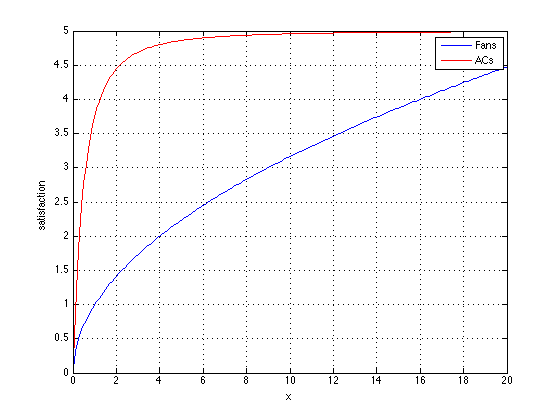
\includegraphics[width=4in]{cvx_assgn_grph1.png}
\caption{Satisfactions for single user}
\end{figure}

\subsubsection{Satisfaction for Multiple Users and Global Satisfaction}
In a room with multiple users, satisfaction \emph{per user} should be of the form $f(x/n)$.
This is justified as about $n$ fans being on in a room with $n$ people amounts to the same satisfaction per user in a room with a single user and single fan on.

Since total user satisfaction in a room doesn't add linearly (assumption 1(d) from the problem statement), we'll use the following functions to measure total satisfaction in a room. Here $x$ represents sum of how much all fans or ACs are turned on in a room and $n$ represents users in the room.
\begin{description}
\item[For fans]: $S_a(x,n) = n^{0.9}s_a(x/n)$
\item[For ACs]: $S_f(x,n) = n^{0.9}s_f(x/n)$
\end{description}

We'll sum these for all the rooms and for all hours.
Thus, Global satisfaction which is our objective function is

\[
S(X^f,X^a) = \sum_{r = 1}^{n_1} \sum_{t=1}^{24} \left [ S_f(X^f_{rt},N_{rt}) + S_a(X^a_{rt},N_{rt}) \right ]
\]
where $N =  O^TU$ is $n_1 \times 24$ matrix representing users in each room at a given hour.

\subsection{Constraints}
Since number of fans in a room are limited, $X^f_{rt}$ is limited by number of fans times $v_f$. 
Similar constraint exists for ACs. 

Therefore 
\begin{eqnarray}
X^f &\leq v_f.F\mathbbm{1}^T_{24}\\
X^a &\leq v_a.A\mathbbm{1}^T_{24}
\end{eqnarray}

Also total energy is given to be constrained by $P$.  Thus
\begin{eqnarray}
\mathbbm{1}^T_{n_1}(y_f.X^f + y_a.X^a + y_c.N)\mathbbm{1}_{24} \leq P
\end{eqnarray}

where $\mathbbm{1}_c$ is a $c \times 1$ column vector with $1$ as all elements and $\leq$ in constraints 1 and 2 is element-wise.

\subsection{Optimization Problem}

Thus, our final optimization problem is 

\begin{equation*}
\begin{aligned}
& \underset{X^f,X^a \geq 0}{\text{maximize}}
& & \sum_{r = 1}^{n_1} \sum_{t=1}^{24} \left [ S_f(X^f_{rt},N_{rt}) + S_a(X^a_{rt},N_{rt}) \right ] \\
& \text{subject to}
& & X^f \leq v_f.F\mathbbm{1}^T_{24}\\
&&& X^a \leq v_a.A\mathbbm{1}^T_{24}\\
&&& \mathbbm{1}^T_{n_1}(y_f.X^f + y_a.X^a + y_c.N)\mathbbm{1}_{24} \leq P
\end{aligned}
\end{equation*}


Objective function is concave because $S_a(x,n) = n^{0.9}(x/n)^p$ ($0 < p < 1$) and 
$S_f(x,n) = cn^{0.9}\left(1- \left (\frac{d}{x/n+d}\right )^2\right)$ are concave in the domain $x\geq 0$.
Since constraints are linear, therefore convex, the whole problem is a convex problem.

\end{document}